\documentclass[]{article}
\usepackage{lmodern}
\usepackage{amssymb,amsmath}
\usepackage{ifxetex,ifluatex}
\usepackage{fixltx2e} % provides \textsubscript
\ifnum 0\ifxetex 1\fi\ifluatex 1\fi=0 % if pdftex
  \usepackage[T1]{fontenc}
  \usepackage[utf8]{inputenc}
\else % if luatex or xelatex
  \ifxetex
    \usepackage{mathspec}
  \else
    \usepackage{fontspec}
  \fi
  \defaultfontfeatures{Ligatures=TeX,Scale=MatchLowercase}
\fi
% use upquote if available, for straight quotes in verbatim environments
\IfFileExists{upquote.sty}{\usepackage{upquote}}{}
% use microtype if available
\IfFileExists{microtype.sty}{%
\usepackage{microtype}
\UseMicrotypeSet[protrusion]{basicmath} % disable protrusion for tt fonts
}{}
\usepackage[margin=1in]{geometry}
\usepackage{hyperref}
\hypersetup{unicode=true,
            pdftitle={Untitled},
            pdfauthor={Daniel Hsiao},
            pdfborder={0 0 0},
            breaklinks=true}
\urlstyle{same}  % don't use monospace font for urls
\usepackage{graphicx,grffile}
\makeatletter
\def\maxwidth{\ifdim\Gin@nat@width>\linewidth\linewidth\else\Gin@nat@width\fi}
\def\maxheight{\ifdim\Gin@nat@height>\textheight\textheight\else\Gin@nat@height\fi}
\makeatother
% Scale images if necessary, so that they will not overflow the page
% margins by default, and it is still possible to overwrite the defaults
% using explicit options in \includegraphics[width, height, ...]{}
\setkeys{Gin}{width=\maxwidth,height=\maxheight,keepaspectratio}
\IfFileExists{parskip.sty}{%
\usepackage{parskip}
}{% else
\setlength{\parindent}{0pt}
\setlength{\parskip}{6pt plus 2pt minus 1pt}
}
\setlength{\emergencystretch}{3em}  % prevent overfull lines
\providecommand{\tightlist}{%
  \setlength{\itemsep}{0pt}\setlength{\parskip}{0pt}}
\setcounter{secnumdepth}{5}
% Redefines (sub)paragraphs to behave more like sections
\ifx\paragraph\undefined\else
\let\oldparagraph\paragraph
\renewcommand{\paragraph}[1]{\oldparagraph{#1}\mbox{}}
\fi
\ifx\subparagraph\undefined\else
\let\oldsubparagraph\subparagraph
\renewcommand{\subparagraph}[1]{\oldsubparagraph{#1}\mbox{}}
\fi

%%% Use protect on footnotes to avoid problems with footnotes in titles
\let\rmarkdownfootnote\footnote%
\def\footnote{\protect\rmarkdownfootnote}

%%% Change title format to be more compact
\usepackage{titling}

% Create subtitle command for use in maketitle
\newcommand{\subtitle}[1]{
  \posttitle{
    \begin{center}\large#1\end{center}
    }
}

\setlength{\droptitle}{-2em}
  \title{Untitled}
  \pretitle{\vspace{\droptitle}\centering\huge}
  \posttitle{\par}
  \author{Daniel Hsiao}
  \preauthor{\centering\large\emph}
  \postauthor{\par}
  \predate{\centering\large\emph}
  \postdate{\par}
  \date{November 12, 2018}

\usepackage{placeins}
\usepackage{siunitx}
\usepackage{multirow}
\usepackage{booktabs}

\begin{document}
\maketitle

{
\setcounter{tocdepth}{3}
\tableofcontents
}
\newpage

\section{Methodology}\label{methodology}

\subsection{Standard Approach}\label{standard-approach}

Consider the two variable case here for illustration purpose. We have
two forecasts, \(y_1\) and \(y_2\), of the true variable \(y\). We want
to combine \(y_1\) and \(y_2\) with a weight \(w\) that we have
\(y_c = w y_1 + (1-w) y_2\). Assume they follow some distribution, e.g.
\(y_1 \sim D(0,\sigma_1)\), \(y_2 \sim D(0,\sigma_2)\), and
\(corr(y_1,y_2)=\rho\). Then the variance of the combined forecast
\(y_c\) is

\begin{equation}
\label{eqn: var yc}
Var(y_c) = w^2\sigma_1^2+ (1-w)^2\sigma_2^2+2w(1-w)\sigma_1\sigma_2\rho,
\end{equation}

and the optimal weight with minimal variance is

\begin{equation}
\label{eqn: simple weight}
w^*=\frac{\sigma_2^2-\sigma_1\sigma_2\rho}{\sigma_1^2+\sigma_2^2 -2\sigma_1\sigma_2\rho}.
\end{equation}

Equation \ref{eqn: simple weight} is the standard benchmark approach in
the combination theory, where extensive research had been done on.
\textbf{add research}. Equation \ref{eqn: simple weight} has a few
empirical results that are against this approach. Two common
alternatives are diagonal covariance matrix and equal weights.

Ignoring the correlation term \(\rho\) by setting \(\rho=0\), we get the
inverse relation on the variance

\begin{equation}
\label{eqn: simple weight no corr}
w^*=\frac{\sigma_2^2}{\sigma_1^2+\sigma_2^2}.
\end{equation}

This is a robust way to avoid the estimation of the covariance when the
dimension goes up. The amount of parameter to estimate for the
covariance with dimension \(n\) is \(\frac{1}{2}n(n+1)\), which is
quadratic in \(n\). When the user only estimates the variances, the
amount of parameter to estimate reduces to \(n\), which greatly
decreases the estimation error. \textbf{add citation}

Equal weights is another common approach that works better empirically.
\textbf{add citation} The forecast combination is in this case just an
arithmetric mean of all forecasts. The reason behind this is the fact
that estimating weights increases or shifts the forecast errors due to
additional estimation error in the estimation of \(w\). We laborate on
the estimation error of \(w\) more later.

\textbf{add more on equal weight}

\subsection{\texorpdfstring{With estimation error of
\(w\)}{With estimation error of w}}\label{with-estimation-error-of-w}

We can also consider the weight as non-deterministic, but related with
\(y\), e.g., in a trivairate distribution with finite third and fourth
moments. Under trivariate distribution, the variance of the weights
influences the expected value and the variance of the combined forecast.
The expected value and the variance of the combined forecast becomes

\begin{equation}
\label{eqn: E & var yc w/ var w}
\begin{aligned}
  E(y_c) =& \mu + (cov(w, y_1-y_2))^2\\
var(y_c) =& E(w)^2\sigma_1^2 + (1-E(w))^2\sigma_2^2 + 2E(w)(1-E(w))\rho\sigma_1\sigma_2 \\
+& E[(w-E(w))(y_1-y_2) (E(w)y_1 + (1-E(w))y_2 - \mu)] \\
+& E[(w-E(w))^2 (y_1-y_2)^2] - cov(w,y_1-y_2)^2.
\end{aligned}
\end{equation}

Equation \ref{ eqn: E & var yc w/ var w} shows the general case of the
forecast combination. If the covariance between \(w\) and \(y_1-y_2\) is
not \(0\), the forecast is biased when combining, with bias
\(cov(w, y_1-y_2)^2\). The variance also increases from euqation
\ref{eqn: var yc} with
\(E[(w-E(w))(y_1-y_2) (E(w)y_1 + (1-E(w))y_2 - \mu)]+E[(w-E(w))^2 (y_1-y_2)^2] - cov(w,y_1-y_2)^2\).
\textbf{can we prove that the change in var(yc) is positive? I tried to
prove it but got stuck at
\(E[(w-E(w))(y_1-y_2) (E(w)y_1 + (1-E(w))y_2 - \mu)]+Var((w-Ew)(y_1-y_2))>0\)}.
This case the only requirements are that the individual forecast to be
unbaised and that the weights sum up to 1.

Let \(d = (d_1, d_2)'\) be the third moment between \(y_1\), \(y_2\),
and
\(\begin{bmatrix} \sigma_{11} & \sigma_{12}\\ \sigma_{12} & \sigma_{22}\end{bmatrix}\)
be the (co)variance matrix, we have

\begin{equation}
\label{eqn: w w/ var w}
\begin{aligned}
w^\dagger = w^*(1+\frac{\sigma_{22} d_1 + \sigma_{11} d_2 -\sigma_{12} (d_1 + d_2)}{\sigma_{11}\sigma_{22} - 2\sigma_{12}}) - \frac{\sigma_{22} d_1 - \sigma{12}d_2}{\sigma_{11}\sigma_{22} - 2\sigma_{12}}.
\end{aligned}
\end{equation}

The non-deterministic weight selection is a linear combination of the
original weight. The non-deterministic weight does not change if the
third moment is \(0\).

\subsection{Negative weights}\label{negative-weights}

Looking back to equation \ref{eqn: simple weight}, we examin the effect
of high correlation term. Assume without loss of generality that
\(\sigma_1 =\sigma_2 (1 + \delta)\), where \(\delta>0\), we rewrite the
weight as

\begin{equation}
\label{eqn: w high corr}
w = \frac{\sigma_2^2(-\rho\delta+ (1-\rho))}{\sigma_1^2+\sigma_2^2 -2\sigma_1\sigma_2\rho}.
\end{equation}

The numerator in \(w\) consist of \(\sigma_2^2\) scaled with a weighted
mean between \(-\delta\) and \(1\) with weight \(\rho\). When \(\rho\)
is small, the weights is close to equation
\ref{eqn: simple weight no corr}. When \(\rho\) is large, the negative
difference in variance \(-\delta\) takes over and results in negative
weights. The level of negativity accounts for both the negtaive
difference and correlation. The boundary case is

\begin{equation}
\label{eqn: corr boundary}
\rho = \frac{\sigma_2}{\sigma_1},
\end{equation}

which \(w\) decreases to \(0\) and \(y_c = y_2\).

From equation \ref{eqn: w w/ var w}, we look in the scaling parameter
and the intercept adjustment vector. Under same condition where
\(\sigma_1 =\sigma_2 (1 + \delta)\), we rewrite the determinant to

\begin{equation}
\sigma_{11}\sigma_{22} - 2\sigma_{12} = \sigma_22 ((1+\delta)^2 - 2 (1+\delta)),
\end{equation}

and the scaling factors

\begin{equation}
\label{eqn: scaling factors}
\begin{aligned}
\frac{\sigma_{22} d_1 - \sigma{12}d_2}{\sigma_{11}\sigma_{22} - 2\sigma_{12}} =& \frac{d_1-\rho(1+\delta) d_2}{(1+\delta)^2 - 2 (1+\delta)}\\
\frac{\sigma_{22} d_1 + \sigma_{11} d_2 -\sigma_{12} (d_1 + d_2)}{\sigma_{11}\sigma_{22} - 2\sigma_{12}} =& \frac{d_1(1- \rho(1+\delta)) + d_2 ((1+\delta)^2-\rho(1+\delta)} {(1+\delta)^2 - 2 (1+\delta))}
\end{aligned}
\end{equation}

\textbf{and I'm lost in what I want to say}

\subsection{Truncated weights}\label{truncated-weights}

To avoid the high correlated forecasts, we use truncation on the
variable. The weight estimation is as follows

\begin{equation}
\label{eqn: w trunc}
** insert latex equation of truncation**
\end{equation}

where the sum of the weights are rescaled to 1.

Assume that there is no skewness in the joint distribution, e.g.,
\(w^*\) is unbiased estimator of the true \(w\). The expected value of
the weights \(\tilde{w}\) is

\begin{equation}
\label{eqn: E w trunc}
\begin{aligned}
E(\tilde{w}) &= E(I_{w>c, w<1-c}w + I_{w>1-c})\\
&=\int_c^{1-c} wf(w)\,\mathrm{d}w+\int_c^{1-c} f(w)\,\mathrm{d}w.
\end{aligned}
\end{equation}

The bias is therefore

\begin{equation}
\label{eqn: bias w trunc}
\begin{aligned}
E(\tilde{w}) - E(w^*) &= \int_{-\infty}^{c} -wf(w)\,\mathrm{d}w+\int_{1-c}^{\infty} (1-w)f(w)\,\mathrm{d}w,
\end{aligned}
\end{equation}

In the first term, we have \(w<c<0\), which cancels out the negative
sign and becomes positive. In the second term we have \(w>1-c>1\), which
gives a negative value in \(1-w\). In general case where \(w\) can go
above \(1-c\) or below \(c\) and the skewness of \(w\) is not 0, the
bias is non-zero. This increases MSE to the estimated \(y_c\).

The variance is

\begin{equation}
\label{eqn: var w trunc}
\begin{aligned}
Var(\tilde{w}) &= E(\tilde{w}^{2})-E(\tilde{w})^2\\
&=E[\tilde{w}^2],
\end{aligned}
\end{equation}

And the change in variance is

\begin{equation}
\label{eqn: delta var w trunc 1}
\begin{aligned}
Var(\tilde{w}) - Var(w) &=\int_{-\infty}^{c} -w^2f(w)\,\mathrm{d}w+\int_{1-c}^{\infty} (1-w^2)f(w)\,\mathrm{d}w \\
& - (\int_c^{1-c} wf(w)\,\mathrm{d}w + \int_{1-c}^{\infty} f(w)\,\mathrm{d}w)^2 + (\int_{-\infty}^{\infty} wf(w)\,\mathrm{d}w)^2.
\end{aligned}
\end{equation}

By Cauchy--Schwarz inequality, and take \(g(w)\) as the weight
generating function of \(\tilde{w}\), we have

\begin{equation}
\label{eqn: delta var w trunc 2}
\begin{aligned}
Var(\tilde{w}) - Var(w) &\leq \int_{-\infty}^{c} -w^2f(w)\,\mathrm{d}w+\int_{1-c}^{\infty} (1-w^2)f(w)\,\mathrm{d}w \\
& - (\int_c^{\infty} g(w)f(w)\,\mathrm{d}w)^2 + \int_{-\infty}^{\infty} w^2f^2(w)\,\mathrm{d}w.
\end{aligned}
\end{equation}

Since \(|g(w)|\leq|w|\) for all \(w\), thus \(g^2(w) \leq w^2\) for all
\(w\). Equation \ref{eqn: delta var w trunc 2} becomes

\subsection{Bias Correction}\label{bias-correction}

Assume for the prediction error from forecast \(i\),
\(\epsilon_i = y - y_i\), that we can decompose it into predictable term
and unpredictable term:

\begin{equation}
\label{eqn: w bias assumption}
\epsilon_i = b_i + \xi_i. 
\end{equation}

Then we can write the weight as a function that minimize the

\section{Survey of Professional Forecasters
(SPF)}\label{survey-of-professional-forecasters-spf}

To illustrate the empirical results, we use the data from ECB
\textbf{(footnote link to data)} in this paper. The data, SPF, is a
quarterly survey initiated by ECB, with the aim to obtain future
estimates on inflation (HICP), RGDP and unemployment rate (UNEM) from
the private sector. Every quarter, a gourp of professional forecasters
from financial and non-financial instutition, such as economic research
institutions, respond to the survey with the idea on the future
economic. Starting 1999, SPF is the longest survey of macroeconomic
expectation in the euro area. Until the date of this paper, there are 75
quarters of observation available, with 1999 Q4 as the first forecasted
value, and 2018 Q2 as the last observed true macroeconomic indice.

The set up of the survey consist of multiple magnitudes of questions,
ranging from different horizon to different distribution. The
forecaststers are asked to provide their point forecast and the
probability of a certain scenario to happen. The survey enables ECB to
do quantitative assessment on the consensus of the market, like the
distribution statistics and standard deviations. For this paper, we take
the 2 most answered time periods, which is 1 year ahead and 2 year ahead
as our data set for all HICP, RGDP, and UNEM.

To compare the forecasts with the actual macroeconomics, we obtain the
true value from ECB data base \textbf{(footnote link to data)}. The data
cannot be observed from the economic in 100\% accuracy within the first
time frame, and exihibits changes to the initial estimates after
revision. We use the final estimate of the macroeconomics where
possible. The use of final estimate is fine is due to the fact that the
original forecast is not the real target to be forecasts.

Within the datasets, not all forecasters did a forecast every time
period. To avoid singular outliers, we remove all forecasters with a
total forecasted period of less than 24 quarter (6 years). The removal
approach is inline with \textbf{(ref paper)}.

Following \textbf{(ref paper)}, we calculate the covariance by looking
at the intersection between each forecasters.

\begin{equation}
\label{equation}
\sigma_{i,j} = \frac{1}{|y_i \cap y_j|}\sum_{k\in \{y_i \cap y_j\}} (y_{i,k}-E(y_i))*(y_{j,k}-E(y_j))
\end{equation}

When there are no intersection between 2 forecasters, we set the
covariance value to 0. Additionally, we calculate the correlation by
using the covariance divided by the standard deviation. Standard
deviation is obtained from the square root of the diagonal.

\begin{equation}
\label{eqn: cov2cor}
\rho_{i,j} = \frac{\sigma_{i,j}}{\sigma_{i}\sigma_{j}}
\end{equation}

The cleaned up gives us a preliminary view on the SPF data without the
noises.

\begin{figure}[!h]
%\centering
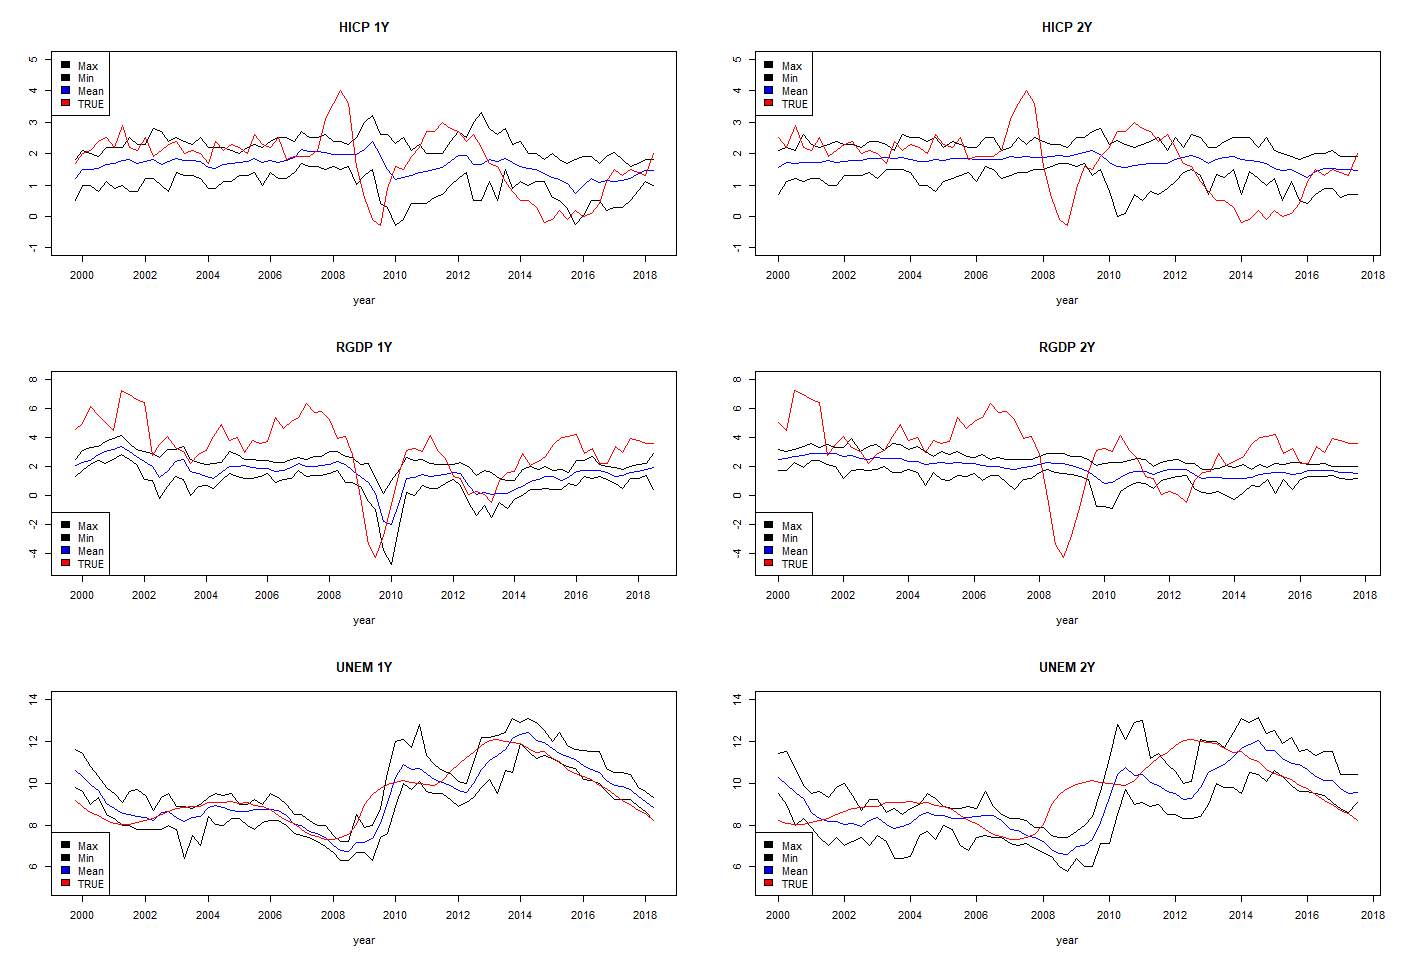
\includegraphics{./Output/Images/SPF.png}
\caption{Survey of Professional Forecasters data illustration}\label{fig: SPF data illustration}
\end{figure}

In figure \ref{fig: SPF data illustration} and table
\ref{tab: correlation summary statistics} we show the plots of the
forecasts along side with the true value in the macroeconomics and the
statistics of the covariance of the forecast error. To avoid too many
lines on the figure by plotting all forecasts, we plot only the minimum,
mean, and maximum from the forecasts. We see that there exist a high
consistency across all forecasts, with two years ahead stronger than one
year. The consistency in the forecast is lower in UNEM than the other
two. Furthermore, many true values lies outside of the forecast range,
with RGDP the worse of all three. More values outside of the forecast
range suggest that restricting positive weights may be a strong
limitation in the forecast combination.

We examine the amount of true value out side of forecast range by
looking at the summary statistics. Let the \(ms\) be an indicator with 1
when the true value is outside of the forecast range, and 0 when the
true value is inside. Table \ref{tab: modelspace summary statistics}
shows the mean of the indicator. From the three macro topic, RGDP with
18\% has the least chance within the forecast range, followed by HICP
with 52\%. UNEM with 62\% has the highest chance to be in the forecast
range. Changing from 1 year to 2 year generally does not influence the
mean of the indicator a lot. From the results from figure
\ref{fig: SPF data illustration} and table
\ref{tab: modelspace summary statistics}, we expect to have large effect
using truncation in the forecast of RGDP, while HICP and UNEM does not
have too strong effect. We also expect the two year ahead forecast will
be better than the one year ahead.

\begin{table}[!h]
\centering
\caption{Mean of the model space indicator of the forecast. The indicators are split up into different forecast topics and different forecast horizons. From the three macro topic, RGDP has the least chance within the forecast range, followed by HICP. UNEM has the highest chance to be in the forecast range.}
\label{tab: modelspace summary statistics}
\begin{tabular}{lcccccc}
\hline
&\multicolumn{6}{c}{Model Space Indicator}\\
\cmidrule{2-7}
Macro topic & \multicolumn{2}{c}{HICP} & \multicolumn{2}{c}{RGDP} & \multicolumn{2}{c}{UNEM} \\
\cmidrule{2-3} \cmidrule{4-5}\cmidrule{6-7}
Horizon     & 1 year & 2 year & 1 year & 2 year & 1 year & 2 year \\ 
\cmidrule{2-2} \cmidrule{3-3} \cmidrule{4-4} \cmidrule{5-5} \cmidrule{6-6} \cmidrule{7-7}
Mean        & 0.45        & 0.51         & 0.83        & 0.82        & 0.37         & 0.39       \\
\hline
\end{tabular}
\end{table}

The table \ref{tab: correlation summary statistics} tell us on how the
forecast error are correlated. The correlation are split up into
different forecast topics and different forecast horizons. Diagonal
element of the correlation matrix is not within the correlation when
generating the summary statistics. For all of the series, the
correlations are on average above 60\%. In HICP and UNEM the correlation
increases across all statistics when the forecast horizon increases,
while RGDP remains the same. The lowest correlation to be found is
-0.02, but this number is not too different than the minimum correlation
in the other two topics.

\begin{table}[!h]
\centering
\caption{Summary statistics of the correlation of the forecast error. The correlation are split up into different forecast topics and different forecast horizons. For all of the series, the correlation are on average above 60\%. In HICP and UNEM the correlation increases across all statistics when the forecast horizon increases, while RGDP remains the same.}
\label{tab: correlation summary statistics}
\begin{tabular}{lcccccc}%{S[table-format=3.2]}
\hline
&\multicolumn{6}{c}{Correlation}\\
\cmidrule{2-7}
Macro topic & \multicolumn{2}{c}{HICP} & \multicolumn{2}{c}{RGDP} & \multicolumn{2}{c}{UNEM} \\
\cmidrule{2-3} \cmidrule{4-5}\cmidrule{6-7}
Horizon     & 1 year & 2 year & 1 year & 2 year & 1 year & 2 year \\ 
\cmidrule{2-2} \cmidrule{3-3} \cmidrule{4-4} \cmidrule{5-5} \cmidrule{6-6} \cmidrule{7-7}
Minimum     & 0.03        & 0.02        & 0.11        & 0.13        & -0.02        & 0.08       \\
First Q     & 0.53        & 0.62        & 0.63        & 0.65        & 0.47         & 0.56       \\
Mean        & 0.64        & 0.70        & 0.75        & 0.75        & 0.59         & 0.67       \\
Median      & 0.66        & 0.72        & 0.81        & 0.80        & 0.62         & 0.70       \\
Third Q     & 0.77        & 0.81        & 0.89        & 0.87        & 0.74         & 0.80       \\
Maximum     & 0.96        & 0.97        & 0.98        & 0.98        & 0.94         & 0.95       \\ 
\hline
\end{tabular}
\end{table}

Analysis on the simple weights given by equation
\ref{eqn: simple weight} provides us a preliminary understanding on the
variability. Table \ref{tab: simple weight summary statistics} shows the
summary statistics of the weight. We see that for all macroeconomic
topics, the mean and median variate around 0.02, which is close to the
calculation from equal weights. Looking at the first and the third
quantile, we see that half of the weights are between -0.6 and 0.6,
which gives us an possible range of effectiveness of the truncation. The
minimum and the maximum is extreme consider that 1 is 100\%. With
negativity up to -11, -21, and -14, and first and third quartile only up
to -0.6 and 0.6, the weight indicates a strong thick tail behaviour.
Looking further to the difference between 1 year and 2 year ahead, we
see that in two out of three macro topics, we see that the extreme
values converge to 0, while RGDP becomes worse. On the other hand, the
gap between first and the third quantile increases for all topics. This
indicates the increase in the choice of negative weights in the general
cases for 2 year horizon. The mean and median does not change much in
relation to the forecsat horizon.

\begin{table}[!h]
\centering
\caption{Summary statistics of the weights from equation \ref{eqn: simple weight}. The mean and median is close to the value from equal weights. However, extreme values exist in the weights, visible in the mimum and maximum. Based on the first and the third quantile, we see that half of the weights are between -0.6 and 0.6.}
\label{tab: simple weight summary statistics}
\begin{tabular}{lcccccc}%{S[table-format=3.2]}
\hline
&\multicolumn{5}{c}{Weights}\\
\cmidrule{2-7}
Macro topic & \multicolumn{2}{c}{HICP} & \multicolumn{2}{c}{RGDP} & \multicolumn{2}{c}{UNEM} \\
\cmidrule{2-3} \cmidrule{4-5}\cmidrule{6-7}
Horizon     & 1 year & 2 year & 1 year & 2 year & 1 year & 2 year \\ 
\cmidrule{2-2} \cmidrule{3-3} \cmidrule{4-4} \cmidrule{5-5} \cmidrule{6-6} \cmidrule{7-7}
Minimum      & -11.05      & -6.21      & -9.00      & -21.79      & -14.41      & -5.64      \\
First Q      & -0.30       & -0.59      & -0.20      & -0.63       & -0.28       & -0.40      \\
Mean         & 0.04        & 0.04       & 0.01       & -0.01       & 0.03        & 0.05       \\
Median       & 0.05        & 0.03       & 0.04       & 0.01        & 0.04        & 0.03       \\
Third Q      & 0.41        & 0.60       & 0.25       & 0.82        & 0.39        & 0.43       \\
Maximum      & 12.94       & 7.56       & 8.74       & 16.34       & 11.26       & 7.90       \\ 
\hline
\end{tabular}
\end{table}

We conclude in for the analysis of SPF that there exhibits
characteristics that are not in the standard cases. By incorporating the
possiblity of negative weights, we expect to see some improvement in the
forecast errors.

\section{Empirical Results}\label{empirical-results}

\subsection{Proceure}\label{proceure}

We seek to evaluate the effect of truncating the weights with SPF data.
The procedure to get the weights can be different between different
researcher. Therefore we provide a through order of the steps we take in
the weight estimation. We do the weights estimation for the truncation
using the following steps:

Given each time to forecast, we take all the know observation before
that forecast time period.

\begin{enumerate}
\def\labelenumi{\arabic{enumi}.}
\item
  Find the nearest positive definite covariance matrix. This step is
  required for the covariance to be invertible. We employ the nearPD
  function from r package \emph{Matrix}. The nearPD function first
  decompose the covariance into univariate variance and the correlation.
  The function then uses the algorithm by \emph{higham} on the
  correlation matrix to compute the nearest positive definite matrix.
  THe final results the the covariance matrix that is combined from the
  univariate variance and the correlation matrix.
\item
  Subset the covariance. Since there are more forecsaters in the
  estimation step than the amount of forecasters in the testing period,
  we take the sub matrix containing only the avaiable forecast on the
  testing period. That is, if 80 forecasters had made some forecasts
  before, but out of them, only 60 has a forecast this time, we discard
  the 20 extra forecasters.
\item
  Estimate the simple weight \(w^*\) from equation
  \ref{eqn: simple weight}.
\item
  Truncate the weights with equation \ref{eqn: w trunc}. The weight no
  has less values and does not sum to one. Due to the fact that our
  selection of the truncation parameter are negative, the summation is
  higher than one and we scale down the weights accordingly.
\item
  Combine the forecast using the weights.
\end{enumerate}

\subsection{Ratio of Mean Squared Prediction
Error}\label{ratio-of-mean-squared-prediction-error}

We eavluate the performance of different weights by mean squared
prediction error (MSPE). The trunacted MSPE is then compared with the
MSPE from equal weight. The results of HICP, RGDP, and UNEM are given in
table \ref{tab: MSPE HICP}, \ref{tab: MSPE RGDP}, and
\ref{tab: MSPE UNEM} respectively. The MSPE of equal weight is not
influenced by the changes in the truncation value. We see in table
\ref{tab: MSPE HICP} that for truncation value

\begin{table}[!h]
\centering
\caption{Mean Squared Prediction Error (MSPE) of inflation with different truncated value. The MSPE of the truncated value is given in the ratio of tuncation to euqal weights. Larger than 1 means truncated is worse, where as smaller than 1 means truncated weight helps in reducing MSPE.}
\label{tab: MSPE HICP}
\begin{tabular}{lcccc}
\hline
          & \multicolumn{4}{c}{HICP}                                                \\
          \cmidrule{2-5}
          & \multicolumn{2}{c}{1 Year Horizon} & \multicolumn{2}{c}{2 Year Horizon} \\
          \cmidrule{2-3} \cmidrule{4-5}
Threshold & Truncated Ratio    & Equal MSPE    & Truncated Ratio    & Equal MSPE    \\
\cmidrule{1-1} \cmidrule{2-2} \cmidrule{3-3} \cmidrule{4-4} \cmidrule{5-5}
-$\infty$ & 3.29               & 0.74          & 2.21               & 1.47          \\
-10       & 2.82               & 0.74          & 2.21               & 1.47          \\
-9        & 2.82               & 0.74          & 2.21               & 1.47          \\
-8        & 2.82               & 0.74          & 2.21               & 1.47          \\
-7        & 2.82               & 0.74          & 2.21               & 1.47          \\
-6        & 2.82               & 0.74          & 2.08               & 1.47          \\
-5        & 2.82               & 0.74          & 2.11               & 1.47          \\
-4        & 2.82               & 0.74          & 2.15               & 1.47          \\
-3        & 2.82               & 0.74          & 1.55               & 1.47          \\
-2        & 0.81               & 0.74          & 0.99               & 1.47          \\
-1        & 0.88               & 0.74          & 0.98               & 1.47          \\
0         & 0.98               & 0.74          & 0.98               & 1.47          \\ 
\hline
\end{tabular}
\end{table}

\begin{table}[!h]
\centering
\caption{Mean Squared Prediction Error (MSPE) of economic growth with different truncated value. The MSPE of the truncated value is given in the ratio of tuncation to euqal weights. Larger than 1 means truncated is worse, where as smaller than 1 means truncated weight helps in reducing MSPE.}
\label{tab: MSPE RGDP}
\begin{tabular}{lcccc}
\hline
          & \multicolumn{4}{c}{RGDP}                                                \\
          \cmidrule{2-5}
          & \multicolumn{2}{c}{1 Year Horizon} & \multicolumn{2}{c}{2 Year Horizon} \\
          \cmidrule{2-3} \cmidrule{4-5}
Threshold & Truncated Ratio    & Equal MSPE    & Truncated Ratio    & Equal MSPE    \\
\cmidrule{1-1} \cmidrule{2-2} \cmidrule{3-3} \cmidrule{4-4} \cmidrule{5-5}
-$\infty$ & 1.44 & 3.54 & 6.07 & 3.36 \\
-10       & 1.44 & 3.54 & 2.64 & 3.36 \\
-9        & 1.44 & 3.54 & 1.03 & 3.36 \\
-8        & 1.09 & 3.54 & 1.03 & 3.36 \\
-7        & 1.1  & 3.54 & 1.02 & 3.36 \\
-6        & 1.1  & 3.54 & 1.06 & 3.36 \\
-5        & 1.1  & 3.54 & 1.07 & 3.36 \\
-4        & 1.15 & 3.54 & 1.09 & 3.36 \\
-3        & 0.88 & 3.54 & 1.08 & 3.36 \\
-2        & 0.84 & 3.54 & 1.08 & 3.36 \\
-1        & 0.86 & 3.54 & 1.14 & 3.36 \\
0         & 0.97 & 3.54 & 1.01 & 3.36 \\ \hline
\end{tabular}
\end{table}

\begin{table}[!h]
\centering
\caption{Mean Squared Prediction Error (MSPE) of nemployment with different truncated value. The MSPE of the truncated value is given in the ratio of tuncation to euqal weights. Larger than 1 means truncated is worse, where as smaller than 1 means truncated weight helps in reducing MSPE.}
\label{tab: MSPE UNEM}
\begin{tabular}{lcccc}
\hline
          & \multicolumn{4}{c}{UNEM}                                                \\
          \cmidrule{2-5}
          & \multicolumn{2}{c}{1 Year Horizon} & \multicolumn{2}{c}{2 Year Horizon} \\
          \cmidrule{2-3} \cmidrule{4-5}
Threshold & Truncated Ratio    & Equal MSPE    & Truncated Ratio    & Equal MSPE    \\
\cmidrule{1-1} \cmidrule{2-2} \cmidrule{3-3} \cmidrule{4-4} \cmidrule{5-5}
-$\infty$ & 1.16 & 0.33 & 4.35 & 0.81 \\
-10       & 1.02 & 0.33 & 4.35 & 0.81 \\
-9        & 1.02 & 0.33 & 4.35 & 0.81 \\
-8        & 1.02 & 0.33 & 4.35 & 0.81 \\
-7        & 1.02 & 0.33 & 4.35 & 0.81 \\
-6        & 1.02 & 0.33 & 4.35 & 0.81 \\
-5        & 1.02 & 0.33 & 2.32 & 0.81 \\
-4        & 0.89 & 0.33 & 2.25 & 0.81 \\
-3        & 0.93 & 0.33 & 1.95 & 0.81 \\
-2        & 0.77 & 0.33 & 1.87 & 0.81 \\
-1        & 0.73 & 0.33 & 1.42 & 0.81 \\
0         & 0.93 & 0.33 & 0.88 & 0.81 \\ \hline
\end{tabular}
\end{table}

\subsection{Out-of-sample truncation
selection}\label{out-of-sample-truncation-selection}

In this section we show the forecast ability in weight truncation when
the truncation parameter is selected out-of-sample (OOS). To perform the
OOS selection of the truncation parameter, we follow the following step:

\begin{enumerate}
\def\labelenumi{\arabic{enumi}.}
\item
  Estimate the normal weight in equation \ref{eqn: simple weight}.
\item
  Calculate the mean squared error (MSE) with truncated weight. The
  truncation parameter ranges from 0 to -10 with a step of -0.1.
\item
  Select the truncation parameter with the lowest MSE. If there are
  multiple truncation points with the same MSE value, we take the
  largest truncation value within the same MSE.
\item
  Use the selected truncation parameter to forecast the combined
  prediction.
\end{enumerate}

A remark on the selection of the largest truncation value. The reason to
choose largest value is that the threshold is closer to the next
changing point. Assume for exmaple, a weight with minimum of -1 is
optimal, and any higher weight results in higher MSE. Then all
truncation values between -10 and -1 gives the same minimal MSE. We
therefore choose -1 to record. The choice does not influence the
forecast, and is pure for the analysis later.

\subsection{Out-of-sample truncation
result}\label{out-of-sample-truncation-result}

We evaluate the OOS forecast ability using the same way as the MSPE with
in-sample truncation parameter selection. The MSPE ratio and the MSPE of
the equal weight is given in table \ref{tab: oos mspe}.

We see in table \ref{tab: oos mspe} that the truncation improves in all
cases from the equal weights. The truncation works better in RGDP 1 year
ahead forecast and UNEM 1 and 2 year ahead forecasts. If we compare the
value to non truncated MSPE, we see that the truncation improves the
forecasts of RGDP 2 year ahead for a large amount. On the other hand,
there is relatively smaller improvement to UNEM 1 year and RGDP 1 year
ahead. This results verify the idea that the truncation in general
improves the upon equal weights even if the truncation uncertainty can
increase the MSPE.

\begin{table}[!h]
\centering
\caption{Mean squared prediction error ratio when the selection of the truncation is also out-of-sample. On average the truncation improves the forecast in all cases.}
\label{tab: oos mspe}
\begin{tabular}{lcccccc}
\hline
&\multicolumn{5}{c}{MSPE with OOS Truncation}\\
\cmidrule{2-7}
Macro topic & \multicolumn{2}{c}{HICP} & \multicolumn{2}{c}{RGDP} & \multicolumn{2}{c}{UNEM} \\
\cmidrule{2-3} \cmidrule{4-5}\cmidrule{6-7}
Horizon     & 1 year & 2 year & 1 year & 2 year & 1 year & 2 year \\ 
\cmidrule{2-2} \cmidrule{3-3} \cmidrule{4-4} \cmidrule{5-5} \cmidrule{6-6} \cmidrule{7-7}
MSPE-ratio  & 0.97   & 0.96   & 0.93   & 0.96   & 0.92   & 0.88   \\ 
\hline
\end{tabular}
\end{table}

To understand the oos truncation more, table
\ref{tab: truncation summary statistics} looks at the selection of the
truncation. The results shows that on average, a truncation around -0.5
is selected, indicating a positive effect on the negative weights. HICP
2 year and RGDP 2 years select on average lower truncation, -0.8 and
-1.0 respectively. UNEM selects -0.2 on average, highest among all. The
minimum across all macro topics are at most -1, with RGDP 1 year, RGDP 2
year, and UNEM 1 year the lowest selected minimum. The first and the
third quantile show that for the most cases, the truncation are not
extreme, ranging between -0.5 to -0.2 in 1 year and -1 to 0 in 2 year
horizon. We notice an increase in the variation when the horizon
increases. This can be attibute to the uncertainty in the horizon adds
uncertainty in the truncation parameter selection.

\begin{table}[!h]
\centering
\caption{Summary statistics of the truncation selected.}
\label{tab: truncation summary statistics}
\begin{tabular}{lcccccc}%{S[table-format=3.2]}
\hline
&\multicolumn{5}{c}{Truncation}\\
\cmidrule{2-7}
Macro topic & \multicolumn{2}{c}{HICP} & \multicolumn{2}{c}{RGDP} & \multicolumn{2}{c}{UNEM} \\
\cmidrule{2-3} \cmidrule{4-5}\cmidrule{6-7}
Horizon     & 1 year & 2 year & 1 year & 2 year & 1 year & 2 year \\ 
\cmidrule{2-2} \cmidrule{3-3} \cmidrule{4-4} \cmidrule{5-5} \cmidrule{6-6} \cmidrule{7-7}
Minimum     & -1.0        & -2.1        & -3.3        & -4.6        & -3.0        & -1.0        \\
First Q     & -0.6        & -1.0        & -0.5        & -1.1        & -0.4        & -0.3        \\
Mean        & -0.5        & -0.8        & -0.5        & -1.0        & -0.4        & -0.2        \\s
Median      & -0.4        & -0.6        & -0.2        & -0.4        & -0.2        & -0.2        \\
Third Q     & -0.3        & -0.3        & -0.1        & -0.2        & -0.2        & 0.0         \\
Maximum     & 0.0         & 0.0         & 0.0         & 0.0         & 0.0         & 0.0         \\ 
\hline
\end{tabular}
\end{table}

\subsection{Bias weighting}\label{bias-weighting}

The bias weighting is an interesting case here. If the model in the bias
estimation successfully estimates the predictable part and the
unpredictable error, this can attirbute to a better weight selection
with additional information gained. We estimate the bias by the
following equation

\begin{equation}
\epsilon_i = b_i + \xi_i.
\end{equation}


\end{document}
